\typeout{(body.tex)}

\begin{frame}
    \titlepage
\end{frame}

\section{number bases}

\subsection{introduction}
\begin{frame}{base-10 numbers}
\begin{eqnarray*}
    12345 &=& 1\cdot10^4 + 2\cdot10^3 + 3\cdot 10^2 + 2\cdot 10^1 + 1\cdot 10^0 \\
    987.65 &=& 9\cdot10^2 + 8\cdot10^1 + 7\cdot10^0 + 6\cdot 10^{-1} + 5\cdot 10^{-2} \\
\end{eqnarray*}
\end{frame}

\begin{frame}{base-2 numbers}
\begin{eqnarray*}
    20_\text{TEN} & = & 11101_\text{TWO} \\
                  & = &1\cdot2^4 + 1\cdot2^3 + 1\cdot2^2 + 0\cdot2^1 + 1\cdot2^0 \\
    4_\text{TEN} & = & 100_\text{TWO}  \\
                 & = & 1\cdot 2^2 + 0\cdot 2^1 + 0\cdot 2^0 \\
    1.25_\text{TEN} & = & 1.01_\text{TWO} \\
                    & = & 1\cdot2^0 + 0\cdot 2^{-1} + 1\cdot2^{-2} \\
\end{eqnarray*}
\end{frame}

\begin{frame}{base-16 numbers}

{\tt
\begin{tabular}{llll llll llll llll}
    0 & 1 & 2 & 3 &
    4 & 5 & 6 & 7 &
    8 & 9 & A & B &
    C & D & E & F \\
\end{tabular}
    }
\begin{flalign*}
    15_\text{TEN} & = & \mathtt{F}_\text{SIXTEEN} & = & 15\cdot16^0 \\
    100_\text{TEN} & = & \mathtt{64}_\text{SIXTEEN} & = & 6\cdot16^1 + 4\cdot16^0 \\
    0.5_\text{TEN} & = & \mathtt{0.8}_\text{SIXTEEN} & = & 8\cdot16^{-1} \\
\end{flalign*}
\end{frame}

\begin{frame}[fragile,label=numCpp]{integers in C++}
\begin{tabular}{l|l}
$15_\text{TEN}$ & \texttt{15} \\
$17_\text{EIGHT}$ & \texttt{017} \\
$\mathtt{F}_\text{SIXTEEN}$ & \texttt{0xF} \\
    \multicolumn{2}{l}{} \\
$99_\text{TEN}$ & \texttt{99} \\
$143_\text{EIGHT}$ & \texttt{0143} \\
$63_\text{SIXTEEN}$ & \texttt{0x63} \\

    \multicolumn{2}{l}{} \\
$16_\text{TEN}$ & \texttt{16} \\
$20_\text{EIGHT}$ & \texttt{020} \\
$10_\text{SIXTEEN}$ & \texttt{0x10} \\
\end{tabular}
\end{frame}


%\begin{comment}
\begin{frame}{last time}
    \begin{itemize}
    \item classes
        \begin{itemize}
        \item declarations in {\tt .h} file
        \item {\tt ClassName::method}
        \item {\tt class ... \{...\}\myemph{;}}
        \item {\tt const}, {\tt static}
        \end{itemize}
    \item objects --- values, not references
        \begin{itemize}
        \item {\tt return Foo(1)} --- {\tt Foo(1)} is temporary Foo object
        \item {\tt x = y} --- copy {\tt x} into {\tt y}
        \end{itemize}
    \item the preprocessor --- {\tt \#define}, {\tt \#include}, etc.
    \item started pointers
    \end{itemize}
\end{frame}
\end{comment}

\begin{comment}
\begin{frame}{last time}
    \begin{itemize}
    \item pointers
        \begin{itemize}
        \item memory --- array of bytes
        \item pointers --- indices into array --- addresses
        \item {\tt T *} --- pointer to T type
        \item {\tt *somePointer} --- use thing at address `pointed to'
        \item {\tt \&someVariable} --- address of someVariable
            \begin{itemize}
            \item AKA ``pointer to'' someVariable
            \end{itemize}
        \end{itemize}
    \item started {\tt new}/{\tt delete}
    \end{itemize}
\end{frame}
\end{comment}

\begin{comment}
\begin{frame}[fragile,label=lastTime]{last time}
\lstset{language=C++,style=small}
    \begin{itemize}
    \item arrays in C++
        \begin{itemize}
        \item \lstinline|int foo[100];|
        \item \lstinline|int *foo = new int[100]; ... delete[] foo;|
        \item \lstinline|foo[42]|
        \end{itemize}
    \item references
        \begin{itemize}
        \item \lstinline|int &refToX = x;|
        \item \lstinline|refToX = valueToAssignToX;|
        \item \lstinline|funcNeedingInt(refToX);|
        \item automatically dereferenced pointers
        \end{itemize}
    \item references as function arguments/pass (started)
    \end{itemize}
\end{frame}

\begin{frame}{SDAC note-taking assistence}
    \begin{itemize}
    \item Student Disability Access Center website ---
        \begin{itemize}
        \item \url{https://studenthealth.virginia.edu/sdac}
        \item ``Notetaker Application'' link
        \end{itemize}
    \end{itemize}
\end{frame}
\end{comment}

\begin{frame}[fragile,label=lastTime]{last time}
\lstset{language=C++,style=small}
    \begin{itemize}
    \item references to const
    \item default methods and destructors
        \begin{itemize}
            \item \lstinline|Foo::Foo()| --- default constructor
            \item \lstinline|Foo::Foo(const Foo& other)| --- copy constructor
            \item \lstinline|Foo::~Foo()| --- destructors
            \item \lstinline|Foo &Foo::operator=(const Foo& other)| --- assignment
        \end{itemize}
    \item overriding operators
        \begin{itemize}
            \item \lstinline|operator>>|, \lstinline|opreator<<| for \lstinline|cin|, \lstinline|cout|
            \item \lstinline|operator+|, \lstinline|operator+=| for \lstinline|string|
            \item \ldots
        \end{itemize}
    \item \lstinline|operator<<|, etc. as method or global function
    \end{itemize}
\end{frame}


\subsection{conversion between bases}

\begin{frame}{terminology}
    \begin{itemize}
    \item base-$X$ number --- $X$ is the \myemph{radix}
    \item I will call components of base $X$ number `digits'
        \begin{itemize}
        \item but not a great term --- digit sometimes implies base-10
        \item sometimes ``radit''
        \item base-2 digit = bit
        \item base-16 digit = nibble (sometimes)
        \end{itemize}
    \item base-10 = decimal
    \item base-2 = binary
    \item base-8 = octal
    \item base-16 = hexadecimal
    \end{itemize}
\end{frame}

\begin{frame}{convert to decimal}
\begin{eqnarray*}
    42_\text{FIVE} & = & \onslide<2->{4 \cdot 5^1 + 2 \cdot 5^0} \\
                   & \onslide<2->{=} & \onslide<3->{20_\text{TEN} + 2 = 22_\text{TEN}} \\
                   ~\\
    121_\text{THREE} & = & \onslide<4->{1\cdot 3^2 + 2 \cdot 3^1 + 1 \cdot 3^0} \\
                     & \onslide<4->{=} & \onslide<5->{9 + 6 + 1 = 16_\text{TEN}} \\
\end{eqnarray*}
\end{frame}

\begin{frame}{convert to something (1)}
\begin{eqnarray*}
    42_\text{TEN} \text{~as radix 5} &=& \only<2>{\_\_\myemph<2>{2}}\only<3>{\_\myemph<3>{3}2}\only<4->{\myemph<4>{1}32_\text{FIVE}} \\
    ~ \\
    \onslide<2->{42 \div 5} & \onslide<2->{=} & \onslide<2->{8 + \ldots} \\
    \onslide<2->{42 \text{~mod~} 5} & \onslide<2->{=} & \onslide<2->{2} \\
    \onslide<2->{42} & \onslide<2->{=} & \onslide<2->{8 \cdot 5 + \myemph<2>{2}} \\
    \onslide<3->{8} & \onslide<3->{=} & \onslide<3->{1 \cdot 5 + \myemph<3>{3}} \\
    \onslide<4->{\myemph<4>{1}}
\end{eqnarray*}
\end{frame}


\begin{frame}{convert to something (2)}
\begin{eqnarray*}
    121_\text{TEN} \text{~as radix 11} &=& \only<2>{\_\_\myemph<2>{0}_\text{ELEVEN}}\only<3>{\_\myemph<3>{0}0_\text{ELEVEN}}%
    \only<4->{\myemph<4>{1}00_\text{ELEVEN}} \\
    ~ \\
    \onslide<2->{121 \div 11} & \onslide<2->{=} & \onslide<2->{11} \\
    \onslide<2->{121 \text{~mod~} 11} & \onslide<2->{=} & \onslide<2->{0} \\
    \onslide<2->{121} & \onslide<2->{=} & \onslide<2->{11 \cdot 11 + \myemph<2>{0}} \\
    \onslide<3->{11} & \onslide<3->{=} & \onslide<3->{1 \cdot 11 + \myemph<3>{0}} \\
    \onslide<4->{\myemph<4>{1}}
\end{eqnarray*}
\end{frame}

\begin{frame}{special case: base-16 to base-2}
    \begin{itemize}
        \item each ``nibble'' (hexadecimal digit) = 4 binary bits
    \end{itemize}
\begin{eqnarray*}
    uz_\text{SIXTEEN} &=& u\cdot 16^1 + z\cdot 16^0 \\
    &=& (u_3\cdot2^3+u_2\cdot2^2+u_1\cdot2^1+u_0\cdot2^0)2^4 + z_3\cdot2^3+\ldots \\
    &=& u_3\cdot2^7+u_2\cdot2^6+u_1\cdot2^5+u_0\cdot2^4+z_3\cdot2^3+\ldots \\
    &=&\left(u_3u_2u_1u_0z_3z_2z_1z_0\right)_\text{TWO}
\end{eqnarray*}
\end{frame}
\begin{frame}{special case: base-16 to base-2}
    \begin{itemize}
        \item each ``nibble'' (hexadecimal digit) = 4 binary bits
    \end{itemize}
\hrule
    \vspace{.5cm}

\begin{tabular}{l|l|l|l}
    \myemph<3>{$\mathtt{1}$} & \myemph<4>{$\mathtt{2}$} & $\mathtt{3}$ & $\mathtt{4}_\text{SIXTEEN}$ \\
    \onslide<2->{\myemph<3>{$\mathtt{0001}$}} & \onslide<2->{\myemph<4>{$\mathtt{0010}$}} & \onslide<2->{$\mathtt{0011}$} & \onslide<2->{$\mathtt{0100}_\text{TWO}$} \\
\end{tabular}

    \vspace{1cm}

\begin{visibleenv}<5->
\begin{tabular}{l|l|l|l}
    $\mathtt{1101}$ & $\mathtt{1110}$ & $\mathtt{0011}$ & $\mathtt{0000}_\text{TWO}$ \\
    \onslide<6->{$\mathtt{C}$} & \onslide<6->{$\mathtt{D}$} & \onslide<6->{$\mathtt{3}$} & \onslide<6->{$\mathtt{0}_\text{SIXTEEN}$} \\
\end{tabular}
\end{visibleenv}
\end{frame}

\begin{frame}{a note on bytes}
    \begin{itemize}
        \item one byte = one ``octet'' = \\
             \myemph<2>{two nibbles} (hexadecimal digits) = \\
             \myemph<3>{eight bits}
        \vspace{.5cm}
        \item this class --- byte is always eight bits
            \begin{itemize}
                \item (some very old machines called different sizes ``bytes'')
            \end{itemize}
    \end{itemize}
\end{frame}


% FIXME: radix conversion exercises?

% FIXME: math in different radix
\begin{frame}{exercise}
    \begin{itemize}
    \item $17_\text{NINE} = ?_\text{SEVEN}$
    \item<2> $17_\text{NINE} = 7 + 9 = 2\cdot 7 + 2$
    \item<2> $17_\text{NINE} = 22_\text{SEVEN}$
    \end{itemize}
\end{frame}

\begin{frame}[fragile,label=otherBase]{on math in other bases}
    \begin{itemize}
    \item you can do math in other bases
    \item usually makes most sense for base 2\ldots
    \end{itemize}
\begin{tabular}{llllll}
    ~ &~   & \small$1$   & \small$1$  &  \small$1$  & ~  \\
    ~& $1$ & $2$ & $3$ &  $4$ & $4_\text{SIXTEEN}$ \\
    ~& $\times$ & ~ & ~ & $1$ & $5_\text{SIXTEEN}$ \\ \hline
    ~   &$5$  & $\mathtt{B}$ & $0$  & $5$  & $4$ \\
    $1$ & $2$ & $3$ & $4$ & $4$ & \\ \hline
    $1$ & $7$ & $\mathtt{E}$  & $4$  &  $9$  & $4_\text{SIXTEEN}$ \\
\end{tabular}
\begin{lstlisting}[language={}]
$ python3 -c 'print("{:x}".format(0x12344*0x15))'
17e494
\end{lstlisting}
\end{frame}


% original slides:
    % Eniac: decimal representation
    % binary representation
    % binary sizes

\section{integer representation (unsigned)}

\begin{frame}{integer representation}
    \begin{itemize}
        \item modern machine represent integers as series of \myemph{bits} (base-2)
        \item why not base-10?
    \end{itemize}
\end{frame}

\begin{frame}{ENIAC: base-10 representation}
\begin{tikzpicture}
\node (eniacPic) {
    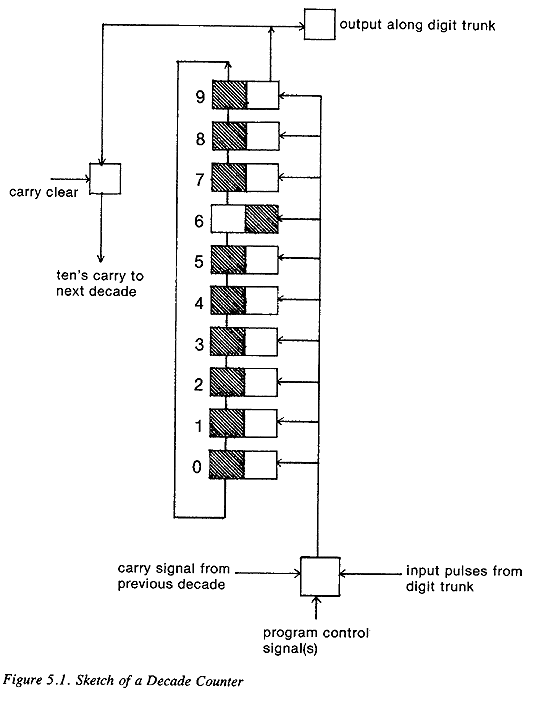
\includegraphics[width=7cm]{Reckoners-fig-05-01}
};
    \node[right=-2cm of eniacPic,align=left] {
        ENIAC: 1946 computer \\
        stored base-10 digits \\
        ~ \\
        ``ring counter'' of ten \\
        electronic switches per digit \\
   };
\begin{visibleenv}<2>
\draw[red,very thick,fill=red,fill opacity=0.05] ([xshift=2.5cm,yshift=-2.5cm]eniacPic.north west) rectangle ++(1.5cm,-1cm);
    \node[red,anchor=south west,inner sep=0mm,fill=white] at ([xshift=4.05cm,yshift=-2.7cm]eniacPic.north west) { flipped switch indicates digit stored };
\end{visibleenv}

\begin{visibleenv}<3>
    \node[red,anchor=south west,inner sep=0mm,fill=white,
        align=left] at ([xshift=4.05cm,yshift=-2cm]eniacPic.north west) {tens of vacuum tubes total \\(each $\sim$1¼\textquotedbl diameter by 2¾\textquotedbl height) };
\end{visibleenv}
\end{tikzpicture}
\end{frame}

% FIXME: base-2 switches

\begin{frame}{base-2 representation}
    \begin{itemize}
    \item base 2 --- each switch represents one ``digit''
        \begin{itemize}
        \item much more efficient use of switches
        \end{itemize}
    \item used in some pre-ENIAC electronic computers
        \begin{itemize}
        \item Atanasoff-Berry computer (1937, Ohio State)
        \item Z3 (1941, German Laboratory for Aviation)
        \end{itemize}
    \item<2-> why not used in ENIAC?
        \begin{itemize}
            \item \fontsize{8}{9}Eckert (ENIAC designer), 1953: ``Although [binary-based digit counters] were known at the time of the construction of the ENIAC, it was not used because it required stable resistors, which were then much more expensive than they are now.''
            \item also, important to input/output decimal digits directly
        \end{itemize}
    \end{itemize}
\imagecredit{quote: ``A Survey of Digital Computer Memory Systems'', Proceedings of the Institute of Radio Engineers, October 1953}
\end{frame}

\begin{frame}{base-2 bit addition}
\begin{tabular}{l|ll}
\textbf{+} & 0 & 1 \\
0 & 0 & \myemph<2>{1} \\
1 & \myemph<2>{1} & \myemph<2>{1} \myemph<3>{carry 1} \\
\end{tabular}
\begin{itemize}
\item<2-> any set to 1 --- result is 1; otherwise 0
\item<3-> both set to 1 --- carry is 1; otherwise 0
\end{itemize}
\end{frame}

\begin{frame}{base-2 capacity}
\begin{eqnarray*}
\text{$n$-bit number:}&\;&b_{n-1}b_{n-2}b_{n-3}\ldots b_2b_1b_0 \\
    & = & \sum_{i=0}^{n-1} b_i \cdot 2^i \\
    & \le & \sum_{i=0}^{n-1} 1 \cdot 2^i = \myemph<2>{2^{n-1}} \\
\end{eqnarray*}
\begin{itemize}
\item<3-> missing pieces:
    \begin{itemize}
    \item negative numbers?
    \item non-whole numbers?
    \item \myemph<4>{what is $n$?}
    \end{itemize}
\end{itemize}
\end{frame}

\begin{frame}{integer size in C++}
\begin{itemize}
\item varies between machines
    \begin{itemize}
    \item compiler uses what makes most sense on each machine?
    \end{itemize}
\end{itemize}
\begin{tabular}{l|l|l}
~ & \multicolumn{2}{c}{size in bits} \\
type & \myemph<3>{minimum} & on lab machines \\
\texttt{\myemph<2>{unsigned} char} & \myemph<3>{8} &  8 \\
\texttt{\myemph<2>{unsigned} short} & \myemph<3>{16} &  16 \\
\texttt{\myemph<2>{unsigned} int} & \myemph<3>{16} & 32 \\
\texttt{\myemph<2>{unsigned} long} & \myemph<3>{32} & 64 \\
\end{tabular}
\begin{tikzpicture}[overlay,remember picture]
\coordinate (place) at ([yshift=-3cm]current page.center);
\tikzset{
    box/.style={draw=red,fill=white,ultra thick,align=left,at=(place)},
}
\begin{visibleenv}<2>
\node[box] { ``unsigned'' --- can't be negative (no sign) };
\end{visibleenv}
\begin{visibleenv}<3>
\node[box] { minimum size required by standard for all C++ compilers \\
             all allowed to be bigger };
\end{visibleenv}
\end{tikzpicture}
\end{frame}

\begin{frame}[fragile,label=querySize]{querying sizes in C++}
\lstset{language=C++,style=smaller}
\begin{lstlisting}
#include <climits>  // C: <limits.h>
...
ULONG_MAX or UINT_MAX or USHRT_MAX or UCHAR_MAX
// e.g. USHRT_MAX == 65535 on lab machines
\end{lstlisting}
\hrule
\vspace{.5cm}
\begin{lstlisting}
#include <limits>  
...
std::numeric_limits<unsigned long>::max()
    // == ULONG_MAX
...
\end{lstlisting}
\vspace{.5cm}
\hrule
\begin{lstlisting}
sizeof(unsigned long)  // number of *bytes* 
    // == 8 on lab machines
...
\end{lstlisting}
\end{frame}


\section{endianness}


\begin{frame}{numbering bits}
\begin{eqnarray*}
\text{option 1: $n$-bit number:}&\;&b_{n-1}b_{n-2}b_{n-3}\ldots b_2b_1b_0 \\
    & = & \sum_{i=0}^{n-1} b_i \cdot 2^i \\
\text{option 2: $n$-bit number:}&\;&b_{0}b_{1}b_{2}\ldots b_{n-3}b_{n-2}b_{n-1} \\
    & = & \sum_{i=0}^{n-1} b_i \cdot 2^{n-i-1} \\
\end{eqnarray*}
\begin{itemize}
\item<2-> two viable ways to number bits
\item<3-> does it matter which I use?
    \begin{itemize}
    \item do I have a way to ask for bit $i$?
    \end{itemize}
\end{itemize}
\end{frame}

\begin{frame}{numbering bytes}
\begin{eqnarray*}
\text{option 1: 4-byte number:}&\;&B_3B_2B_1B_0 \\
    & = & \sum_{i=0}^{3} B_i \cdot 256^i \\
\text{option 2: 4-byte number:}&\;&B_0B_1B_2B_3 \\
    & = & \sum_{i=0}^{3} b_i \cdot 256^{3-i} \\
\end{eqnarray*}
\begin{itemize}
\item<2-> two viable ways to number bytes
\item<3-> does it matter which I use?
    \begin{itemize}
    \item in memory, yes --- each byte needs an address (number)
    \end{itemize}
\end{itemize}
\end{frame}

\begin{frame}[fragile,label=memoryEnd]{memory}
\begin{tikzpicture}
\matrix[tight matrix,
    column 1/.style={nodes={draw=none,text width=1cm}},
    column 2/.style={nodes={text width=2cm,font=\tt}},
    row 1/.style={nodes={font=\normalfont}},
    label={[font=\bfseries,align=center]north:memory \\ (as 64-bit values)}
] (mem64) {
    addr. \& value (64-bit) \\
    0 \& 123999 \\
    8 \& 323232 \\
    16 \& 434093 \\
    \ldots \& \ldots \\
};
    \node[below=1cm of mem64] {
        $\begin{aligned}
            123999 &=& 1\cdot 256^2 \\
                   &+& 228\cdot 256^1 \\
                   &+& 95 \cdot 256^0 \\
        \end{aligned}$
    };
\begin{visibleenv}<2>
\matrix[tight matrix,
    column 1/.style={nodes={draw=none,text width=1cm}},
    column 2/.style={nodes={text width=1cm,font=\tt}},
    row 1/.style={nodes={font=\normalfont,draw=none}},
    label={[font=\bfseries,align=center]north:if \myemph{little endian} \\ (as 8-bit values)},
    anchor=north west,
] (mem8) at ([xshift=1.25cm]mem64.north east) {
    addr. \& value (8-bit) \\
    0 \& 95 \\
    1 \& 228 \\
    2 \& 1 \\
    3 \& 0 \\
    4 \& 0 \\
    5 \& 0 \\
    6 \& 0 \\
    7 \& 0 \\
    8 \& 160 \\
    9 \& 238 \\
    10 \& 4 \\
    11 \& \ldots \\
    \ldots \& \ldots \\
};
\tikzset{
    hiBox/.style={draw=red,inner sep=0.5mm,ultra thick}
}
\node[hiBox,fit=(mem64-2-2)] {};
\node[hiBox,fit=(mem8-2-2) (mem8-9-2)] {};
\draw[red,ultra thick] (mem64-2-2.north east) -- (mem8-2-2.north west);
\draw[red,ultra thick] (mem64-2-2.south east) -- (mem8-9-2.south west);
\matrix[tight matrix,
    column 1/.style={nodes={draw=none,text width=1cm}},
    column 2/.style={nodes={text width=1cm,font=\tt}},
    row 1/.style={nodes={font=\normalfont,draw=none}},
    label={[font=\bfseries,align=center]north:if \myemph{big endian} \\ (as 8-bit values)},
    anchor=north east,
] (mem8B) at ([xshift=-1.25cm]mem64.north west) {
    addr. \& value (8-bit) \\
    0 \& 0 \\
    1 \& 0 \\
    2 \& 0 \\
    3 \& 0 \\
    4 \& 0 \\
    5 \& 1 \\
    6 \& 228 \\
    7 \& 95 \\
    8 \& 0 \\
    9 \& 0 \\
    10 \& 0 \\
    11 \& \ldots \\
    \ldots \& \ldots \\
};
\tikzset{
    hiBox/.style={draw=red,inner sep=0.5mm,ultra thick}
}
\node[hiBox,fit=(mem64-2-2)] {};
\node[hiBox,fit=(mem8-2-2) (mem8-9-2)] {};
\draw[red,ultra thick] (mem64-2-2.north east) -- (mem8-2-2.north west);
\draw[red,ultra thick] (mem64-2-2.south east) -- (mem8-9-2.south west);
\node[hiBox,fit=(mem8B-2-2) (mem8B-9-2)] {};
\draw[red,ultra thick] (mem64-2-2.north west) -- (mem8B-2-2.north east);
\draw[red,ultra thick] (mem64-2-2.south west) -- (mem8B-9-2.south east);
\end{visibleenv}
\end{tikzpicture}
\end{frame}

\begin{frame}[fragile,label=findEndian]{finding endianness in C++}
\lstset{
    language=C++,
    style=smaller,
     moredelim={**[is][\btHL<all:1>]{@1}{1@}},
     moredelim={**[is][\btHL<all:2-3>]{@2}{2@}},
     moredelim={**[is][\btHL<all:4>]{@3}{3@}},
     moredelim={**[is][\btHL<all:5>]{@4}{4@}},
     moredelim={**[is][\btHL<all:6>]{@5}{5@}},
     moredelim={**[is][\btHL<all:7>]{@6}{6@}},
}
\vspace{-.6cm}
\begin{lstlisting}
#include <iostream>
using std::cout; using std::hex; using std::endl;
int main() {
    unsigned long value = @60x0123456789ABCDEF6@;
    cout << hex << value << endl;
    unsigned char *ptr = @2(unsigned char*) &value2@;
    for (int i = 0; i < sizeof(unsigned long); ++i) {
        cout << (int) @3ptr[i]3@ << " ";
    }
    ...
}
\end{lstlisting}
\hrule
\lstset{
    language={},
    style=smaller,
     moredelim={**[is][\btHL<all:1>]{@1}{1@}},
     moredelim={**[is][\btHL<all:2-3>]{@2}{2@}},
     moredelim={**[is][\btHL<all:4>]{@3}{3@}},
     moredelim={**[is][\btHL<all:5>]{@4}{4@}},
     moredelim={**[is][\btHL<all:6>]{@5}{5@}},
     moredelim={**[is][\btHL<all:7>]{@6}{6@}},
}
little endian (e.g. lab machine):
\vspace{-.15cm}
\begin{lstlisting}
@6123456789abcdef6@
@4ef4@ cd ab 89 67 45 23 1
\end{lstlisting}
\hrule
big endian:
\begin{lstlisting}
@6123456789abcdef6@
@515@ 23 45 67 89 ab cd ef
\end{lstlisting}
\begin{tikzpicture}[overlay,remember picture]
\coordinate (place) at ([yshift=4cm]current page.south);
\tikzset{
    box/.style={draw=red,fill=white,ultra thick,align=left,at=(place),inner sep=2mm},
}
\begin{visibleenv}<2>
\node[box] {
    get pointer to \myemph{byte} with \\ lowest address in \texttt{value}
}; 
\end{visibleenv}
\begin{visibleenv}<3>
\node[box] {
    unless you do something like this \\
    won't see endianness
}; 
\end{visibleenv}
\begin{visibleenv}<4>
\node[box] {
    use pointer to get \texttt{i}th byte of value \\
    (cast to int to output as number, not character)
};
\end{visibleenv}
\begin{visibleenv}<5>
\node[box] {
    little endian: byte 0 is \myemph{least significant} \\
    (affects overall value the least)
};
\end{visibleenv}
\begin{visibleenv}<6>
\node[box] {
    big endian: byte 0 is \myemph{most significant} \\
    (affects overall value the most)
};
\end{visibleenv}
\begin{visibleenv}<7>
\node[box] {
    but we don't write numbers in a different order \\
    based on which end we call ``part 0''
};
\end{visibleenv}
\end{tikzpicture}
\end{frame}

\begin{frame}{little versus big endian}
\begin{itemize}
\item little endian --- least significant part has lowest address
\begin{itemize}
\item i.e. index 0 is the one's place
\end{itemize}
\item big endian --- most significant part has the lowest address
\begin{itemize}
\item i.e. index $n-1$ is the one's place
\end{itemize}
\vspace{.5cm}
\end{itemize}
\end{frame}

\begin{frame}{endianness in the real world}
\begin{itemize}
\item today and this course: little endian is dominant
    \begin{itemize}
    \item e.g. x86, \textit{typically} ARM
    \end{itemize}
\item historically: big endian was dominant
    \begin{itemize}
    \item e.g. \textit{typically} SPARC, POWER, Alpha, MIPS, \ldots
    \item still commonly used for networking because of this
    \end{itemize}
\item many architectures have switchable endianness
    \begin{itemize}
    \item e.g. ARM, SPARC, POWER, MIPS
    \item usually, OS chooses one endianness
    \end{itemize}
\end{itemize}
\end{frame}

\begin{frame}{middle endian}
\begin{itemize}
\item sometimes not just big/little endian
\item e.g. number bytes most to least significant as \\
    5, 6, 7, 8, 1, 2, 3, 4
\item e.g. doubles on little-endian ARM
\item generally some sort of historical accident
    \begin{itemize}
    \item e.g. ARM floating point designed for big endian?
    \end{itemize}
\end{itemize}
\end{frame}

\begin{frame}{endianness is about addresses}
\begin{itemize}
\item endianness is about numbering, \\
    not (necessairily) placement on the page
\item but, probably assume English order (left to right, etc.) if not otherwise specified
\end{itemize}
\begin{tikzpicture}
\matrix[tight matrix,
    column 1/.style={nodes={draw=none,text width=1cm}},
    column 2/.style={nodes={text width=1cm,font=\tt}},
    row 1/.style={nodes={font=\normalfont,draw=none}},
    anchor=north west,
] (mem8A) {
    addr. \& value \\
    0 \& 95 \\
    1 \& 228 \\
    2 \& 1 \\
    3 \& 0 \\
    4 \& 0 \\
    5 \& 0 \\
    6 \& 0 \\
    7 \& 0 \\
    8 \& 160 \\
    9 \& 238 \\
    10 \& 4 \\
    11 \& \ldots \\
    \ldots \& \ldots \\
};
\matrix[tight matrix,
    column 1/.style={nodes={draw=none,text width=1cm}},
    column 2/.style={nodes={text width=1cm,font=\tt}},
    row 1/.style={nodes={font=\normalfont,draw=none}},
    anchor=north west,
    right=3cm of mem8A
] (mem8B) {
    addr. \& value \\
    \ldots \& \ldots \\
    11 \& \ldots \\
    10 \& 4 \\
    9 \& 238 \\
    8 \& 160 \\
    7 \& 0 \\
    6 \& 0 \\
    5 \& 0 \\
    4 \& 0 \\
    3 \& 0 \\
    2 \& 1 \\
    1 \& 228 \\
    0 \& 95 \\
};
\node[font=\Huge] at ($(mem8A)!0.5!(mem8B)$) {=};
\end{tikzpicture}
\end{frame}

\begin{frame}{endianness and bit-order}
    \begin{itemize}
    \item we won't talk about \myemph{bit order}
    \item because bits don't have addresses
    \vspace{.5cm}
    \item if I say ``bit $0$'', question: ``numbering from least significant or most significant''?
        \begin{itemize}
        \item nothing about how pointers, etc. work suggests either answer is correct
        \end{itemize}
    \end{itemize}
\end{frame}

\begin{frame}{endianness and writing out bytes}
    \begin{itemize}
        \item \texttt{0x0102} in binary: \texttt{00000001000000010}
            \begin{itemize}
            \item English's order --- most significant first
            \end{itemize}
        \item bytes of \texttt{0x0102} in big endian: \\(byte 0) \texttt{00000001} (byte 1) \texttt{00000010}
        \item bytes of \texttt{0x0102} in little endian: \\(byte 0) \texttt{00000010} (byte 1) \texttt{00000001}
        \vspace{.5cm}
        \item \textit{usually}, we don't change the order we write bits
        \item if writing out bytes, first in reading order is usually lowest address
            \begin{itemize}
            \item (we'll specify if not)
            \end{itemize}
    \end{itemize}
\end{frame}


%\begin{comment}
\begin{frame}{last time}
    \begin{itemize}
    \item classes
        \begin{itemize}
        \item declarations in {\tt .h} file
        \item {\tt ClassName::method}
        \item {\tt class ... \{...\}\myemph{;}}
        \item {\tt const}, {\tt static}
        \end{itemize}
    \item objects --- values, not references
        \begin{itemize}
        \item {\tt return Foo(1)} --- {\tt Foo(1)} is temporary Foo object
        \item {\tt x = y} --- copy {\tt x} into {\tt y}
        \end{itemize}
    \item the preprocessor --- {\tt \#define}, {\tt \#include}, etc.
    \item started pointers
    \end{itemize}
\end{frame}
\end{comment}

\begin{comment}
\begin{frame}{last time}
    \begin{itemize}
    \item pointers
        \begin{itemize}
        \item memory --- array of bytes
        \item pointers --- indices into array --- addresses
        \item {\tt T *} --- pointer to T type
        \item {\tt *somePointer} --- use thing at address `pointed to'
        \item {\tt \&someVariable} --- address of someVariable
            \begin{itemize}
            \item AKA ``pointer to'' someVariable
            \end{itemize}
        \end{itemize}
    \item started {\tt new}/{\tt delete}
    \end{itemize}
\end{frame}
\end{comment}

\begin{comment}
\begin{frame}[fragile,label=lastTime]{last time}
\lstset{language=C++,style=small}
    \begin{itemize}
    \item arrays in C++
        \begin{itemize}
        \item \lstinline|int foo[100];|
        \item \lstinline|int *foo = new int[100]; ... delete[] foo;|
        \item \lstinline|foo[42]|
        \end{itemize}
    \item references
        \begin{itemize}
        \item \lstinline|int &refToX = x;|
        \item \lstinline|refToX = valueToAssignToX;|
        \item \lstinline|funcNeedingInt(refToX);|
        \item automatically dereferenced pointers
        \end{itemize}
    \item references as function arguments/pass (started)
    \end{itemize}
\end{frame}

\begin{frame}{SDAC note-taking assistence}
    \begin{itemize}
    \item Student Disability Access Center website ---
        \begin{itemize}
        \item \url{https://studenthealth.virginia.edu/sdac}
        \item ``Notetaker Application'' link
        \end{itemize}
    \end{itemize}
\end{frame}
\end{comment}

\begin{frame}[fragile,label=lastTime]{last time}
\lstset{language=C++,style=small}
    \begin{itemize}
    \item references to const
    \item default methods and destructors
        \begin{itemize}
            \item \lstinline|Foo::Foo()| --- default constructor
            \item \lstinline|Foo::Foo(const Foo& other)| --- copy constructor
            \item \lstinline|Foo::~Foo()| --- destructors
            \item \lstinline|Foo &Foo::operator=(const Foo& other)| --- assignment
        \end{itemize}
    \item overriding operators
        \begin{itemize}
            \item \lstinline|operator>>|, \lstinline|opreator<<| for \lstinline|cin|, \lstinline|cout|
            \item \lstinline|operator+|, \lstinline|operator+=| for \lstinline|string|
            \item \ldots
        \end{itemize}
    \item \lstinline|operator<<|, etc. as method or global function
    \end{itemize}
\end{frame}


\section{negative number representation}

\begin{frame}{representing negative numbers}
\vspace{-.5cm}
\begin{tikzpicture}
\tikzset{
    >=Latex,
    myl/.style={font=\small\tt,align=center},
}
\begin{visibleenv}<1-4>
\node at (1.5, 4mm) {unsigned integers};
\draw[thick] (0, 0)  -- (9, 0);
\draw[thick] (0,2mm) -- (0,-2mm) node[below,myl] {0000\ldots0000 \\ = $0$};
\draw[thick] (9,2mm) -- (9,-2mm) node[below,myl] {1111\ldots1111 \\ = $2^n-1$};
\draw[thick] (4.45,2mm) -- (4.45,-2mm);
\draw[thick,dotted] (4.45,-2mm) -- ++(-1cm,-0.2cm) node[below,myl] {0111\ldots1111 \\ = $2^{n-1}-1$};
\draw[thick] (4.5,2mm) -- (4.5,-2mm);
\draw[thick,dotted] (4.5,2mm) -- ++(1cm,0.2cm) node[above,myl] {1000\ldots0000 \\ = $2^{n}-1$};
\end{visibleenv}

\begin{visibleenv}<2->
\begin{scope}[yshift=-5cm]
\node at (1.5, 4mm) {signed integers};
\draw[thick] (0, 0) -- (9, 0);
\draw[thick] (0,2mm) -- (0,-2mm) node[below,myl] {0000\ldots0000 \\ = $0$};
\draw[thick] (9,2mm) -- (9,-2mm) node[below,myl] {1111\ldots1111 \\ = \myemph<5>{???}};
\draw[thick] (4.45,2mm) -- (4.45,-2mm);
\draw[thick] (4.5,2mm) -- (4.5,-2mm);
\draw[thick,dotted] (4.45,-2mm) -- ++(-1cm,-0.2cm) node[below,myl] {0111\ldots1111 \\ = $2^{n-1}-1$};
\draw[thick,dotted] (4.5,2mm) -- ++(1cm,0.2cm) node[above,myl] {1000\ldots0000 \\ = \myemph<5>{???}};
\end{scope}
\end{visibleenv}

\begin{visibleenv}<3>
\draw[blue,ultra thick] (0, 0) -- (4.45, 0);
\draw[blue,ultra thick] (0, -5) -- (4.45, -5);
\draw[blue,->,dashed,thick] (2, -2.5) -- (2, -3mm);
\draw[blue,->,dashed,thick] (2, -2.5) -- (2, -47mm);
\node[fill=white,align=left] at (2.5, -2.5) {positive numbers up to $2^n-1$ \\
            goal: same bits, signed or not};
\end{visibleenv}

\begin{visibleenv}<4>
\draw[green!50!black,ultra thick] (4.5, 0) -- (9, 0);
\draw[green!50!black,ultra thick] (4.5, -5) -- (9, -5);
\draw[green!50!black,->,dashed,thick] (7.5, -2.5) -- (7.5, -3mm);
\draw[green!50!black,->,dashed,thick] (7.5, -2.5) -- (7.5, -47mm);
\node[fill=white,align=left] at (7.5, -2.5) {unsigned: $2^{n-1}$ and bigger \\
                signed: negative numbers, but how?};
\end{visibleenv}

\begin{visibleenv}<5->
\draw[green!50!black,ultra thick] (4.5, -5) -- (9, -5);
\node[draw=black,thin,fill=white,font=\tt\small] at (4.5, 0) {
\begin{tabular}{l|lll}
~ & \normalfont \myemph<6,9>{sign \& magnitude} & \normalfont \myemph<6,8>{1's complement} & \normalfont \myemph<7,8>{2's complement} \\ \hline
000\ldots000 & \myemph<6>{$0$} & \myemph<6>{$0$} & 0 \\
011\ldots111 & $2^{n-1}-1$ &$2^{n-1}-1$ & \myemph<7>{$2^{n-1}-1$} \\
100\ldots000 & \myemph<6>{$0$} & $-2^{n-1}+1$ & \myemph<7>{$-2^{n-1}$} \\
111\ldots111 & \myemph<9>{$-2^{n-1}+1$} & \myemph<6,8>{$0$} & \myemph<8>{$-1$} \\
\end{tabular}
};
\end{visibleenv}

\begin{visibleenv}<6>
\node[red!70!black,align=center] at (4.5, -2.5) {
    two representations of zero? \\
    \texttt{x~==~y} needs to do something special
};
\end{visibleenv}

\begin{visibleenv}<7>
\node[red!70!black,align=center] at (4.5, -2.5) {
    more negative values than positive values?
};
\end{visibleenv}

\begin{visibleenv}<8>
\node[red!70!black,align=center] at (4.5, -2.5) {
    all 1's --- least negative? 
};
\end{visibleenv}

\begin{visibleenv}<9>
\node[red!70!black,align=center] at (4.5, -2.5) {
    all 1's --- most negative?
};
\end{visibleenv}

\end{tikzpicture}
\end{frame}
% FIXME: also hilight ticks in rep slide

% FIXME: concrete 3-bit or 4-bit example?

\begin{frame}{sign and magnitude}
\vspace{-.5cm}
\begin{tikzpicture}
\tikzset{
    >=Latex,
    myl/.style={font=\small\tt,align=center},
}
\begin{visibleenv}<1-2>
\node at (1.5, 4mm) {unsigned integers};
\draw[thick] (0, 0)  -- (9, 0);
\draw[thick] (0,2mm) -- (0,-2mm) node[below,myl] {0000\ldots0000 \\ = $0$};
\draw[thick] (9,2mm) -- (9,-2mm) node[below,myl] {1111\ldots1111 \\ = $2^n-1$};
\draw[thick] (4.45,2mm) -- (4.45,-2mm);
\draw[thick,dotted] (4.45,-2mm) -- ++(-1cm,-0.2cm) node[below,myl] {0111\ldots1111 \\ = $2^{n-1}-1$};
\draw[thick] (4.5,2mm) -- (4.5,-2mm);
\draw[thick,dotted] (4.5,2mm) -- ++(1cm,0.2cm) node[above,myl] {1000\ldots0000 \\ = $2^{n}-1$};
\end{visibleenv}

\begin{visibleenv}<3>
\node[align=left] at (4.5, 0) {
    first bit is ``sign bit'' --- 0 = positive, 1 = negative \\
    flip sign bit to negate number
};
\end{visibleenv}

\begin{visibleenv}<4>
% FIXME: arithmetic
\node[align=left] at (4.5, 0) {
    adding 1 \\ different direction if negative
};
\end{visibleenv}

\begin{scope}[yshift=-5cm]
\draw[thick] (0, 0) -- (9, 0);
\draw[thick] (0,2mm) -- (0,-2mm) node[below,myl] {0000\ldots0000 \\ = $+0$};
\draw[thick] (9,2mm) -- (9,-2mm) node[below,myl] {1111\ldots1111 \\ = $-2^{n-1}+1$};
\draw[thick] (4.45,2mm) -- (4.45,-2mm);
\draw[thick] (4.5,2mm) -- (4.5,-2mm);
\draw[thick,dotted] (4.45,-2mm) -- ++(-1cm,-0.2cm) node[below,myl] {0111\ldots1111 \\ = $2^{n-1}-1$};
\draw[thick,dotted] (4.5,2mm) -- ++(0cm,0.2cm) node[above,myl] {1000\ldots0000 \\ = $-0$};
\begin{visibleenv}<2-3>
\draw[thick, dotted, green!50!black] (.5,0mm) -- ++(0cm,15mm) node[above] {\myemph<2-3>{0}000\ldots0101 = $6$};
\draw[thick, dotted, green!50!black] (5.,0mm) -- ++(2cm,15mm) node[above] {\myemph<2-3>{1}000\ldots0101 = $-6$};
\end{visibleenv}
\begin{visibleenv}<4>
\draw[ultra thick,->,red] (1, 0) -- (1.5, 0);
\draw[ultra thick,->,red] (6, 0) -- (5.5, 0);
\end{visibleenv}
\end{scope}
\end{tikzpicture}
\end{frame}

\begin{frame}{1's complement}
\vspace{-.5cm}
\begin{tikzpicture}
\tikzset{
    >=Latex,
    myl/.style={font=\small\tt,align=center},
}
\begin{visibleenv}<1-2>
\node at (1.5, 4mm) {unsigned integers};
\draw[thick] (0, 0)  -- (9, 0);
\draw[thick] (0,2mm) -- (0,-2mm) node[below,myl] {0000\ldots0000 \\ = $0$};
\draw[thick] (9,2mm) -- (9,-2mm) node[below,myl] {1111\ldots1111 \\ = $2^n-1$};
\draw[thick] (4.45,2mm) -- (4.45,-2mm);
\draw[thick,dotted] (4.45,-2mm) -- ++(-1cm,-0.2cm) node[below,myl] {0111\ldots1111 \\ = $2^{n-1}-1$};
\draw[thick] (4.5,2mm) -- (4.5,-2mm);
\draw[thick,dotted] (4.5,2mm) -- ++(1cm,0.2cm) node[above,myl] {1000\ldots0000 \\ = $2^{n}-1$};
\end{visibleenv}

\begin{visibleenv}<3>
\node[align=left] at (4.5, 0) {
    flip all bits to negate number
};
\end{visibleenv}

\begin{visibleenv}<4>
% FIXME: arithmetic
\node[align=left] at (4.5, 0) {
    adding 1 \\
    same direction, no matter original sign
};
\end{visibleenv}

\begin{scope}[yshift=-5cm]
\draw[thick] (0, 0) -- (9, 0);
\draw[thick] (0,2mm) -- (0,-2mm) node[below,myl] {0000\ldots0000 \\ = $+0$};
\draw[thick] (9,2mm) -- (9,-2mm) node[below,myl] {1111\ldots1111 \\ = $-0$};
\draw[thick] (4.45,2mm) -- (4.45,-2mm);
\draw[thick] (4.5,2mm) -- (4.5,-2mm);
\draw[thick,dotted] (4.45,-2mm) -- ++(-1cm,-0.2cm) node[below,myl] {0111\ldots1111 \\ = $^{n-1}-1$};
\draw[thick,dotted] (4.5,2mm) -- ++(0cm,0.2cm) node[above,myl] {1000\ldots0000 \\ = $-2^{n-1}-1$};
\begin{visibleenv}<2-3>
\draw[thick, dotted, green!50!black] (.5,0mm) -- ++(0cm,15mm) node[above] {0000\ldots0101 = $6$};
\draw[thick, dotted, green!50!black] (5.,0mm) -- ++(2cm,15mm) node[above] {1111\ldots1010 = $-6$};
\end{visibleenv}
\begin{visibleenv}<4>
\draw[ultra thick,->,red] (1, 0) -- (1.5, 0);
\draw[ultra thick,->,red] (5.5, 0) -- (6, 0);
\end{visibleenv}
\end{scope}
\end{tikzpicture}
\end{frame}

% FIXME: more on addition in one's complement?

\begin{frame}{two's complement}
\vspace{-.5cm}
\begin{tikzpicture}
\tikzset{
    >=Latex,
    myl/.style={font=\small\tt,align=center},
}
\begin{visibleenv}<1-2>
\node at (1.5, 4mm) {unsigned integers};
\draw[thick] (0, 0)  -- (9, 0);
\draw[thick] (0,2mm) -- (0,-2mm) node[below,myl] {0000\ldots0000 \\ = $0$};
\draw[thick] (9,2mm) -- (9,-2mm) node[below,myl] {1111\ldots1111 \\ = $2^n-1$};
\draw[thick] (4.45,2mm) -- (4.45,-2mm);
\draw[thick,dotted] (4.45,-2mm) -- ++(-1cm,-0.2cm) node[below,myl] {0111\ldots1111 \\ = $2^{n-1}-1$};
\draw[thick] (4.5,2mm) -- (4.5,-2mm);
\draw[thick,dotted] (4.5,2mm) -- ++(1cm,0.2cm) node[above,myl] {1000\ldots0000 \\ = $2^{n}-1$};
\end{visibleenv}

\begin{visibleenv}<3>
\node[align=left] at (4.5, 0) {
    flip all bits and add 1 to negate number
};
\end{visibleenv}

\begin{visibleenv}<4>
% FIXME: arithmetic
\node[align=left] at (4.5, 0) {
    adding 1 \\
    same direction, no matter original sign
};
\end{visibleenv}

\begin{scope}[yshift=-5cm]
\draw[thick] (0, 0) -- (9, 0);
\draw[thick] (0,2mm) -- (0,-2mm) node[below,myl] {0000\ldots0000 \\ = $+0$};
\draw[thick] (9,2mm) -- (9,-2mm) node[below,myl] {1111\ldots1111 \\ = $-1$};
\draw[thick] (4.45,2mm) -- (4.45,-2mm);
\draw[thick] (4.5,2mm) -- (4.5,-2mm);
\draw[thick,dotted] (4.45,-2mm) -- ++(-1cm,-0.2cm) node[below,myl] {0111\ldots1111 \\ = $2^{n-1}-1$};
\draw[thick,dotted] (4.5,2mm) -- ++(0cm,0.2cm) node[above,myl] {1000\ldots0000 \\ = $-2^{n-1}$};
\begin{visibleenv}<2-3>
\draw[thick, dotted, green!50!black] (.5,0mm) -- ++(0cm,15mm) node[above] {0000\ldots0101 = $6$};
\draw[thick, dotted, green!50!black] (5.,0mm) -- ++(2cm,15mm) node[above] {1111\ldots1010 = $-6$};
\end{visibleenv}
\begin{visibleenv}<4>
\draw[ultra thick,->,red] (1, 0) -- (1.5, 0);
\draw[ultra thick,->,red] (5.5, 0) -- (6, 0);
\end{visibleenv}
\end{scope}
\end{tikzpicture}
\end{frame}

\begin{frame}{2's complement (alt. perspective)}
\begin{tikzpicture}
\tikzset{
    >=Latex,
    myl/.style={font=\small\tt,align=center}
}
\matrix[
    tight matrix noline,
    nodes={text width=1.75cm,minimum height=1cm,align=center,font=\tt\small},
    column 1/.style={nodes={text width=1.75cm,align=left,font=\normalfont\small}},
    column 3/.style={nodes={text width=0.25cm}},
    column 5/.style={nodes={text width=0.25cm}},
    column 7/.style={nodes={text width=0.25cm}},
    column 9/.style={nodes={text width=0.25cm}},
    row 1/.style={nodes={text=green!70!black}},
    row 4/.style={nodes={text=blue!70!black}},
    label={north:2's complement (5 bit)},
] (twosComplEx) {
   +10 = \& \textbf<2>{0} \& \& 1 \& \& 0 \& \& 1 \& \& 0 \\
      \& $0\cdot(-2^{4})$ \& + \& $1\cdot2^3$ \& + \& $0\cdot2^2+$ \& + \& $1\cdot2^1+$ \& + \& $0\cdot2^0$ \\
   ~     \& $0$ \& + \& $2^3$ \& + \& $0$ \& + \& $2^1$ \& + \& $0=10$ \\
   -10 = \& \textbf<2>{1} \& \& 0 \& \& 1 \& \& 1 \& \& 0 \\
        \& $1\cdot(-2^{4})$ \& +\& $0\cdot2^3$ \& + \& $1\cdot2^2$ \& + \& $1\cdot2^1$ \& + \& $0\cdot2^0$ \\
   ~     \& $-2^{4}$ \& + \& $0$ \& +  \& $2^2$ \& + \& $2^1$ \& + \& $0=-10$ \\
};
\begin{visibleenv}<2>
\node[draw=red,ultra thick,fit = (twosComplEx-1-2)] {};
\node[draw=red,ultra thick,fit= (twosComplEx-6-2),label={south:``$-2^4$s place''}] { };
\end{visibleenv}
\end{tikzpicture}
\end{frame}

\begin{frame}
\begin{tikzpicture}
\tikzset{
    >=Latex
}
\node[font=\large\bfseries] at (0, 4.5) {{\color{blue!70!black}unsigned} v. {\color{green!70!black}2's complement}};
\draw[ultra thick,opacity=0.1,black] (0,0) circle (3cm);
\foreach \iu/\ii\pat in {0/0/000,1/1/001,2/2/010,3/3/011,4/-4/100,5/-3/101,6/-2/110,7/-1/111} {
    \node[align=center] (x-\iu) at (90 - 180 / 4 * \ii:3cm) {{\color{blue!70!black}$\iu$} or {\color{green!70!black}$\ii$}\\ {\tt \pat}};
}
\begin{visibleenv}<2-3>
\draw[very thick,red,->] (0, 4) arc (90:90- 180 / 4: 4 and 4) node[midway,above,sloped] {add $1$};
\end{visibleenv}
\begin{visibleenv}<3-3>
\draw[very thick,blue!20!black,dotted,->] (0, 4) arc (90:90- 180 / 4 * 7: 4 and 4) node[pos=0.2,above,sloped] {add {\color{green!70!black}$7$} or {\color{blue!70!black}$-1$}};
\end{visibleenv}

\coordinate (onePtB) at (2.8,2.8);

\begin{visibleenv}<4->
\draw[very thick,red,->] (onePtB) arc (90 - 180/4*1:90- 180 / 4 * 2: 4 and 4) node[midway,above,sloped] {add $1$};
\end{visibleenv}
\begin{visibleenv}<5->
\draw[very thick,blue!20!black,dotted,->] (onePtB) arc (90-180/4*1:90- 180 / 4 * 8: 4 and 4) node[pos=0.3,below,sloped] {add {\color{green!70!black}$7$} or {\color{blue!70!black}$-1$}};
\end{visibleenv}

\begin{visibleenv}<6>
\node[align=left] at (6, 2) {
    2's complement addition \\
    is same as unsigned addition \\
};
\end{visibleenv}
\end{tikzpicture}
\end{frame}

\begin{frame}{converting to 2's complement (version 1)}
\begin{itemize}
\item take absolute value, convert to bits
\item if negative, flip all the bits and add one
\vspace{.5cm}
\item $-14 \rightarrow -00001110 \rightarrow 11110001 + 1 \rightarrow  11110010$
\item $-127 \rightarrow -01111111 \rightarrow 10000000 + 1 \rightarrow 10000001$
\item $-128 \rightarrow -10000000 \rightarrow 01111111 + 1 \rightarrow 10000000$
\hrule
\item if negative, take absolute value, subtract from $2^n$, encode that
\item $-14 \rightarrow 2^8 - 14 = 242 \rightarrow 11110010$
\item $-127 \rightarrow 2^8 - 127 = 129 \rightarrow 10000001$
\item $-128 \rightarrow 2^8 - 127 = 129 \rightarrow 10000000$
\end{itemize}
\end{frame}



% FIXME: two's complement

% FIXME: addition in two's complement --- wraparound

\begin{frame}[fragile,label=twosComplement]{two's complement summary}
\begin{tikzpicture}[visible on=<1->]
\matrix [matrix of nodes,nodes={text width=1.5em,inner xsep=0pt,outer sep=0pt,every label/.style={font=\scriptsize}}] (places) {
    |[label={90:$-2^{31}$}]|1 \& |[label={90:$+2^{30}$}]|1 \& |[label=90:$+2^{29}$]|1 \& \ldots \&  |[label={90:$+2^2$}]| 1 \& |[label={90:$+2^1$}]| 1 \& |[label={90:$+2^0$}]| 1 \\
};
\node[left=1ex of places,yshift=-1ex] (minusOne) {$-1 =$};
\end{tikzpicture}

\begin{tikzpicture}[scale=1.2]
\onslide<2->{
\draw[ultra thick,opacity=0.1,black] (0,0) circle (2cm);
\begin{scope}[every node/.style={font=\scriptsize},outer sep=0pt,inner sep=1pt]
\node[color=red!40!black] (minusOne) at (115:2cm) {$-1$};
\node (zero) at (90:2cm) {$0$};
\node[color=green!40!black] (one) at (65:2cm) {$1$};
\node[color=green!40!black] (intmax) at (300:2cm) {$2^{31}-1$};
\node[color=red!40!black] (intmin) at (270:2cm) {$-2^{31}$};
\node[color=red!40!black] (intmin1) at (240:2cm) {$-2^{31}+1$};
\end{scope}

\draw[green!40!black,dotted,thick,-latex] (60:2cm) arc (60:-50:2cm);
\draw[red!40!black,dotted,thick,-latex] (230:2cm) arc (230:120:2cm);
\draw[red!40!black,thin,-latex] (260:2cm) arc (260:250:2cm);
\draw[thin,-latex] (290:2cm) arc (290:280:2cm);
}
\onslide<3->{
\begin{scope}[every node/.style={font=\tiny,inner sep=1mm,outer sep=0mm}]
\node[below right=1pt of intmax,color=green!40!black] (intmaxDecode) {\lstinline|0111 1111 |\ldots\lstinline| 1111|};
\node[below=3pt of intmin,color=red!40!black] (intminDecode) {\lstinline|1000 0000 |\ldots\lstinline| 0000|};
\node[above left=1pt of minusOne,color=red!40!black] (minusOneDecode) {\lstinline|1111 1111 |\ldots\lstinline| 1111|};
\end{scope}
\draw[thin,black!70!green] (intmax) -- (intmaxDecode);
\draw[thin,black!70!red] (intmin) -- (intminDecode);
\draw[thin,black!70!red] (minusOne) -- (minusOneDecode);
}
\end{tikzpicture}
\end{frame}

% FIXME: exercises


\begin{comment}
\begin{frame}{two's complement exercise}
\begin{itemize}
\item -45 as 8-bit two's complement?
    \begin{itemize}
    \item<2->
        $-45 \rightarrow -00101101_\text{TWO} \rightarrow 11010010 + 1 \rightarrow 11010011$
    \end{itemize}
\item -128 as 8-bit two's complement?
    \begin{itemize}
    \item<2->
        $-128 \rightarrow -10000000_\text{TWO} \rightarrow 01111111 + 1 \rightarrow 10000000$
    \end{itemize}
\item -129 as 8-bit two's complement?
    \begin{itemize}
    \item<2->
        $-129 \rightarrow -10000001_\text{TWO} \rightarrow 01111110 + 1 \rightarrow 01111111$
    \item<2-> \myemph{OVERFLOW} --- result not negative \end{itemize}
\end{itemize}
\end{frame}
\end{comment}



\section{integer overflow}

\begin{frame}{integer overflow}
    \begin{itemize}
    \item ``wrap around''
    \item 8-bit signed: $127 + 1 \rightarrow -128$
    \item 8-bit unsigned: $255 + 1 \rightarrow 0$ 
    \item 16-bit signed: $32\,767 + 1 \rightarrow -32\,768$
    \item 16-bit unsigned: $65\,536 + 1 \rightarrow 0$ 
    \item 32-bit signed: around $2$ billion
    \item 64-bit signed: around $9\times 10^{18}$
    \item \ldots
    \end{itemize}
\end{frame}

% FIXME: possibly skip

\begin{frame}[fragile,label=cppIO1]{on integer overflow in C++ (1)}
\lstset{language=C++,style=small}
\begin{lstlisting}
unsigned int x; // lab machines: 32-bit unsigned
x = 4294967295; // (2 to the 32) minus 1
x += 10;
cout << x << endl; // OUTPUT: 9
\end{lstlisting}
\end{frame}

\begin{frame}[fragile,label=cppIO2]{on integer overflow in C++ (1)}
\lstset{language=C++,style=small}
\begin{lstlisting}
int x; // lab machines: 32-bit signed
x = 2147483647;  // mxaimum integer
x += 10;  // UNDEFINED!
cout << x << endl; // EXPECT big negative number,
                   // but not gaurenteed
\end{lstlisting}
    \begin{itemize}
    \item in practice: usually get wraparound behavior\ldots
    \item but compiler is not required to do this for signed numbers
        \begin{itemize}
        \item and takes advantage of this to optimize, sometimes
        \end{itemize}
    \end{itemize}
\end{frame}



\section{real numbers}

\subsection{introduction/fixed point}
\begin{frame}{some real numbers}
\begin{itemize}
\item $\frac{1}{3}$
\item $-\frac{100}{7}$
\item $\pi$
\item $0.1$
\item $\sqrt{2}$
\item \ldots
\vspace{.5cm}
\item want to represent these: {\small accurately? compactly? efficiently?}
\end{itemize}
\end{frame}

\begin{frame}{fixed point}
\begin{eqnarray*}
\frac{1}{3} &=& 0.101010101\ldots_\text{TWO}  \\\
            &\approx& +0000.1010_\text{TWO} \text{--- represent as {\tt 00000 1010}} \\
\frac{100}{7} &=& 1110.001001001\ldots_\text{TWO}  \\
            &\approx& -1110.0010_\text{TWO} \text{--- represent as {\tt 01110 0010}} \\
\end{eqnarray*}
\begin{itemize}
\item<2-> $x \approx y/2^K$ --- represent with fixed-sized signed integer $y$
\begin{itemize}
    \item this case: $y/2^4$ and $y$ is 9 bits.
\end{itemize}
\end{itemize}
\end{frame}

\begin{frame}{why fixed-point?}
\begin{itemize}
\item $x \approx y/2^K$ ($y$ fixed-sized singed integer)
\item math similar to integer math:
    \begin{itemize}
    \item addition/subtraction --- same
    \item multiplication --- same except divide by $2^K$ 
    \item division --- same except multiply by $2^K$
    \end{itemize}
\item easy to understand what values are represented well
\end{itemize}
\end{frame}

\begin{frame}{why not fixed-point?}
\begin{itemize}
\item pretty small range of numbers for space used
\item hard to choose a $2^K$ that works for lots of applications
\end{itemize}
\end{frame}

\begin{frame}{recall (?): scientific notation}
\begin{eqnarray*}
+\frac{1}{3} &=& +0.33333333\ldots \\
            &\approx& \myemph<3>{+}\myemph<4>{3.33}\cdot \myemph<6>{10}^{\myemph<5>{-1}} \\
-\frac{100}{7} &=& -14.285714\ldots \\
            &\approx& \myemph<3>{-}\myemph<4>{1.42}\cdot \myemph<6>{10}^{\myemph<5>{+1}} \\
\end{eqnarray*}
\begin{itemize}
\item<2-> $\myemph<3>{\pm}\text{\myemph<4>{mantissa}} \cdot \text{\myemph<6>{base}}^\text{\myemph<5>{exponent}}$
\end{itemize}
\end{frame}

\begin{frame}{base-2 scientific notation}
\begin{eqnarray*}
\frac{1}{3} &=& 0.101010101\ldots_\text{TWO}  \\\
            &\approx& 0.1010101010_\text{TWO} =  +1.0101010101_\text{TWO} \cdot 2^-1\\
\frac{100}{7} &=& 1110.001001001\ldots_\text{TWO}  \\\
            &\approx& -1110.0010010_\text{TWO} = -1.1100010010_\text{TWO} \cdot 2^3\\
\end{eqnarray*}
\end{frame}




\subsection{floating point intro: half precision}
\begin{frame}{IEEE half-precision floating point}
\begin{tikzpicture}
\tikzset{
    >=Latex,
    labelLine/.style={draw,thick,dotted},
    myLabel/.style={align=center,font=\small},
    pm/.style={blue!70!black},
    mant/.style={green!60!black},
    expt/.style={orange!80!black},
}
\begin{scope}[every node/.style={inner sep=0mm}]
\node[pm] (pm) {-};
\node[anchor=base west] (onePt) at (pm.base east) {$1.$};
\node[anchor=base west,mant] (mant) at (onePt.base east) {$1100010010_\text{TWO}$};
\node[anchor=base west] (cdot) at (mant.base east) {\cdot};
\node[anchor=base west] (expt) at (cdot.base east) {$2^{\color{orange!80!black}3}$};
\end{scope}
\begin{visibleenv}<2->
\node[pm,below left=1cm of pm,myLabel] (signLabel) {sign (1 bit) };
\node[pm,below=0cm of signLabel,align=left] {
    $0$ for $+$ \\
    $1$ for $-$
};
\draw[pm,labelLine] (pm) -- (signLabel);
\node[mant,right=1.5cm of signLabel,myLabel] (mantLabel) {mantissa ($10$ bits)};
\draw[mant,labelLine] (mant) -- (mantLabel);
\node[mant,below=0cm of mantLabel,align=left] {
    don't store leading ``$1.$'' \\
    (because always present)
};
\node[right=1.5cm of mantLabel,myLabel,expt] (exptLabel) {exponent ($5$ bits)};
\draw[expt,labelLine] (expt) -- (exptLabel);
\node[expt,below=0cm of exptLabel,align=left] {
    store $3+15=18$ \\
    $15$ is `bias'
};
\end{visibleenv}
\begin{visibleenv}<3->
    \node[below=2cm of mantLabel] (value) {
    \tt {\color{blue!70!black}1} {\color{orange!80!black}10010} {\color{green!60!black}1100010010}
};
\end{visibleenv}
\begin{visibleenv}<4->
\node[below=1cm of value,align=left] {
    on typical little endian system: \\
    byte 0: {\tt \color{green!60!black}00010010} \\
    byte 1: {\tt {\color{blue!70!black}1}{\color{orange!80!black}10010}\color{green!60!black}11}
};
\end{visibleenv}
\end{tikzpicture}
\end{frame}

\begin{frame}{IEEE half precision float}
\begin{itemize}
\item 1 sign bit ($1$ for negative)
\item 5 expontent bits
    \begin{itemize}
    \item bias of 15 --- if bits as unsigned are $e$, exponent is $E=e-127$
    \end{itemize}
\item 10 mantissa bits
    \begin{itemize}
    \item leading ``1.'' not stored
    \end{itemize}
\vspace{.5cm}
\item $\text{value} = (1-2\cdot \text{sign}) \cdot (1.\text{mantissa}_\text{TWO}) \cdot 2^{\text{exponent}-15}$
\end{itemize}
\end{frame}



%\begin{comment}
\begin{frame}{last time}
    \begin{itemize}
    \item classes
        \begin{itemize}
        \item declarations in {\tt .h} file
        \item {\tt ClassName::method}
        \item {\tt class ... \{...\}\myemph{;}}
        \item {\tt const}, {\tt static}
        \end{itemize}
    \item objects --- values, not references
        \begin{itemize}
        \item {\tt return Foo(1)} --- {\tt Foo(1)} is temporary Foo object
        \item {\tt x = y} --- copy {\tt x} into {\tt y}
        \end{itemize}
    \item the preprocessor --- {\tt \#define}, {\tt \#include}, etc.
    \item started pointers
    \end{itemize}
\end{frame}
\end{comment}

\begin{comment}
\begin{frame}{last time}
    \begin{itemize}
    \item pointers
        \begin{itemize}
        \item memory --- array of bytes
        \item pointers --- indices into array --- addresses
        \item {\tt T *} --- pointer to T type
        \item {\tt *somePointer} --- use thing at address `pointed to'
        \item {\tt \&someVariable} --- address of someVariable
            \begin{itemize}
            \item AKA ``pointer to'' someVariable
            \end{itemize}
        \end{itemize}
    \item started {\tt new}/{\tt delete}
    \end{itemize}
\end{frame}
\end{comment}

\begin{comment}
\begin{frame}[fragile,label=lastTime]{last time}
\lstset{language=C++,style=small}
    \begin{itemize}
    \item arrays in C++
        \begin{itemize}
        \item \lstinline|int foo[100];|
        \item \lstinline|int *foo = new int[100]; ... delete[] foo;|
        \item \lstinline|foo[42]|
        \end{itemize}
    \item references
        \begin{itemize}
        \item \lstinline|int &refToX = x;|
        \item \lstinline|refToX = valueToAssignToX;|
        \item \lstinline|funcNeedingInt(refToX);|
        \item automatically dereferenced pointers
        \end{itemize}
    \item references as function arguments/pass (started)
    \end{itemize}
\end{frame}

\begin{frame}{SDAC note-taking assistence}
    \begin{itemize}
    \item Student Disability Access Center website ---
        \begin{itemize}
        \item \url{https://studenthealth.virginia.edu/sdac}
        \item ``Notetaker Application'' link
        \end{itemize}
    \end{itemize}
\end{frame}
\end{comment}

\begin{frame}[fragile,label=lastTime]{last time}
\lstset{language=C++,style=small}
    \begin{itemize}
    \item references to const
    \item default methods and destructors
        \begin{itemize}
            \item \lstinline|Foo::Foo()| --- default constructor
            \item \lstinline|Foo::Foo(const Foo& other)| --- copy constructor
            \item \lstinline|Foo::~Foo()| --- destructors
            \item \lstinline|Foo &Foo::operator=(const Foo& other)| --- assignment
        \end{itemize}
    \item overriding operators
        \begin{itemize}
            \item \lstinline|operator>>|, \lstinline|opreator<<| for \lstinline|cin|, \lstinline|cout|
            \item \lstinline|operator+|, \lstinline|operator+=| for \lstinline|string|
            \item \ldots
        \end{itemize}
    \item \lstinline|operator<<|, etc. as method or global function
    \end{itemize}
\end{frame}

\subsection{other IEEE floating point}
\begin{frame}{other IEEE precisions}
\begin{tabular}{l|lll}
~ & half & single & double & quad \\ \hline
C++*/Java type& --- & \texttt{float} & \texttt{double} & ---\\
sign bits & 1 & 1 & 1 & 1\\
exponent bits & 5 & 8 & 11 & 15 \\
exponent bias & 15 {\small ($2^5-1$)} & 127 {\small ($2^7-1$)} & 1023 {\small ($2^{10}-1$)} & 16383 ($2^{14}-1$)\\
mantissa bits & 10 & 23 & 52 & 112\\
total bits & 16 & 32 & 64 & 128\\
\end{tabular}\\
    {\scriptsize (* = typical C++ type; might vary in some implementations)}
\end{frame}




\subsection{converting to/from floating point}
\begin{frame}{diversion: 25.25 to binary}
\begin{eqnarray*}
    25.25 &=& 25+\frac{1}{4} = \frac{101}{4} \\
          &=& \frac{1100101_\text{TWO}}{2^2} \\
          &=& 11001.01_\text{TWO}
\end{eqnarray*}
\end{frame}

\begin{frame}{diversion: 25.25 to binary}
\begin{eqnarray*}
    25.25 &=& 2^4 + (25.25 - 2^4) = 2^4 + 9.25 \\
          &=& 2^4 + 2^3 + (9.25-2^3) = 2^4 + 2^3 + 1.25 \\
          &=& 2^4 + 2^3 + (9.25-2^3) = 2^4 + 2^3 + 1.25 \\
          &~& (1.25 < 2^2) \\
          &~& (1.25 < 2^1) \\
          &=& 2^4 + 2^3 + (1.25-2^0) = 2^4 + 2^3 + 2^0 + 0.25 \\
          &~& (0.25 < 2^{-1}) \\
          &=& 2^4 + 2^3 + 2^0 + 2^{-2} + (0.25 - 2^{-2}) = 2^4 + 2^3 + 2^0 + 2^{-2} \\
\end{eqnarray*}
\end{frame}


\begin{frame}{\texttt{float} example: manually (1)}
\begin{eqnarray*}
    25.25 &=& \frac{101}{4} = \frac{101}{2^2}
\end{eqnarray*}
largest power of two $<25.25$? $16=2^4$ \\
(means $1 < 25.25/16 < 2$)
\begin{eqnarray*}
    \frac{101}{4} \cdot \frac{2^4}{2^4} &=& \frac{101 \cdot 2^4}{2^6} \\
                &=& \frac{101}{2^6}\times 2^4 \\
                &=& \frac{1100101_\text{TWO}}{2^6}\times 2^4 \\
                &=& 1.100101_\text{TWO} \times 2^4
\end{eqnarray*}
\end{frame}

\begin{frame}{\texttt{float} example: manually (2)}
\begin{tikzpicture}
\tikzset{
    >=Latex,
    labelLine/.style={draw,thick,dotted},
    myLabel/.style={align=center,font=\small},
    pm/.style={blue!70!black},
    mant/.style={green!60!black},
    expt/.style={orange!80!black},
}
\node (calc) at (6, 0) { 
    $25.25 = \frac{101}{4} = 11001.01_{\text{TWO}} = $
};
\begin{scope}[every node/.style={inner sep=0mm}]
\node[pm] (pm) at ([yshift=-1cm,xshift=-4cm]calc) {+};
\node[anchor=base west] (onePt) at (pm.base east) {$1.$};
\node[anchor=base west,mant] (mant) at (onePt.base east) {$1001\,0100\,0000\,0000\,0000\,000_\text{TWO}$};
\node[anchor=base west] (cdot) at (mant.base east) {\cdot};
\node[anchor=base west] (expt) at (cdot.base east) {$2^{\color{orange!80!black}4}$};
\end{scope}
\begin{visibleenv}<2->
\node[pm,below left=1cm and -.5cm of pm,myLabel] (signLabel) {sign (1 bit) };
\node[pm,below=0cm of signLabel,align=left,font=\small] {
    $0$ for $+$
};
\draw[pm,labelLine] (pm) -- (signLabel);
\node[mant,right=1cm of signLabel,myLabel] (mantLabel) {mantissa ($23$ bits)};
\draw[mant,labelLine] (mant) -- (mantLabel);
\node[mant,below=0cm of mantLabel,align=left,font=\small] {
    (leading ``$1.$'' not stored)\\
};
\node[right=1.5cm of mantLabel,myLabel,expt] (exptLabel) {exponent ($8$ bits)};
\draw[expt,labelLine] (expt) -- (exptLabel);
\node[expt,below=0cm of exptLabel,align=left,font=\small] {
    store ``$4+127=$\\
    $1000\,0011_\text{TWO}$'' \\
    $127$ is bias for \texttt{float}
};
\end{visibleenv}
\begin{visibleenv}<3->
\node[below=2cm of mantLabel,font=\small\tt] (value) {
    {\color{blue!70!black}0} {\color{orange!80!black}1000$\,$0011} {\color{green!60!black}1001$\,$0100$\,$0000$\,$0000$\,$0000$\,$000}
};
\end{visibleenv}
\end{tikzpicture}
\end{frame}

\begin{frame}[fragile,label=floatUnion]{\texttt{float} example: from C++}
\lstset{
    language=C++,
    style=smaller
}
% FIXME: discussion about union
\begin{lstlisting}
#include <iostream>
using std::cout; using std::hex; using std::endl;
// union: all elements use the *same memory*
union floatOrInt {
    float f;
    unsigned int u;
};
int main() {
    union floatOrInt x;
    x.f = 25.25;
    cout << hex << x.u << endl;
// OUTPUT: 41ca0000
}
\end{lstlisting}
\begin{tikzpicture}
    \matrix[tight matrix noline,nodes={font=\tt,text width=1.5cm,align=center}] {
    4 \& 1 \& c \& a \& 0 \& 0 \& 0 \& 0 \\
    {\color{blue!70!black}0}{\color{orange!80!black}100} \& \color{orange!80!black}0001 \& \color{green!60!black}1100 \& \color{green!60!black}1010 \& \color{green!60!black}0000 \& \color{green!60!black} 0000 \& \color{green!60!black}0000 \& \color{green!60!black}0000 \\
};
\end{tikzpicture}
\end{frame}

\begin{frame}{\texttt{float} example 2: manually}
\begin{tikzpicture}
\tikzset{
    >=Latex,
    labelLine/.style={draw,thick,dotted},
    myLabel/.style={align=center,font=\small},
    pm/.style={blue!70!black},
    mant/.style={green!60!black},
    expt/.style={orange!80!black},
}
\node[align=center] (calc) at (6, 0) { 
    $0.1_\text{TEN} = \frac{1}{16} + 0.0375 = \frac{1}{16} + \frac{1}{32} + 0.00625 = $ \\
    $\frac{1}{16} + \frac{1}{32} + \frac{1}{256} + 0.00234375 = \ldots$ \\
    \strut$\ldots = 0.00011001100110011\ldots_\text{TWO} \myemph<4>{\approx}$ 
};
\begin{scope}[every node/.style={inner sep=0mm}]
\node[pm] (pm) at ([yshift=-2cm,xshift=-4cm]calc) {+};
\node[anchor=base west] (onePt) at (pm.base east) {$1.$};
    \node[anchor=base west,mant] (mant) at (onePt.base east) {$1001\,1001\,1001\,1001\,1001\,10\mathbf{1}_\text{TWO}$};
\node[anchor=base west] (cdot) at (mant.base east) {\cdot};
\node[anchor=base west] (expt) at (cdot.base east) {$2^{\color{orange!80!black}-4}$};
\end{scope}
\begin{visibleenv}<2->
\node[pm,below left=1cm and -.5cm of pm,myLabel] (signLabel) {sign (1 bit) };
\node[pm,below=0cm of signLabel,align=left,font=\small] {
    $0$ for $+$
};
\draw[pm,labelLine] (pm) -- (signLabel);
\node[mant,right=1cm of signLabel,myLabel] (mantLabel) {mantissa ($23$ bits)};
\draw[mant,labelLine] (mant) -- (mantLabel);
\node[mant,below=0cm of mantLabel,align=left,font=\small] {
    last $\mathbf{1}$ from \myemph<4>{rounding}
};
\node[right=1.5cm of mantLabel,myLabel,expt] (exptLabel) {exponent ($8$ bits)};
\draw[expt,labelLine] (expt) -- (exptLabel);
\node[expt,below=0cm of exptLabel,align=left,font=\small] {
    store ``$-4+127=$\\
    $0111\,1011_\text{TWO}$''
};
\end{visibleenv}
\begin{visibleenv}<3->
\node[below=1cm of mantLabel,font=\small\tt] (value) {
    {\color{blue!70!black}0} {\color{orange!80!black}0111$\,$1011} {\color{green!60!black}1001$\,$1001$\,$1001$\,$1001$\,$1001$\,$101}
};
\end{visibleenv}
\begin{visibleenv}<4->
\node[below=0cm of value] {
    \myemph<4>{closest} \texttt{float} to 0.1
    between $0.1$ and $0.1000001$
};
\end{visibleenv}
\end{tikzpicture}
\end{frame}

\begin{frame}{aside: binary long division}
    \includegraphics[height=0.9\textheight]{long-division}
\end{frame}


\begin{frame}[fragile,label=floatEx2In1]{\texttt{float} example 2: inaccurate (1)}
\lstset{
    language=C++,
    style=smaller
}
\begin{lstlisting}
#include <iostream>
using std::cout; using std::endl;

int main(void) {
    int count;
    float base = 0.1f;
    for (count = 0; base * count < 10000000; ++count) {}
    cout << count << endl;
    // OUTPUT: 99999996
    return 0;
}
\end{lstlisting}
\end{frame}

\begin{frame}[fragile,label=floatEx2In2]{\texttt{float} example 2: inaccurate (2)}
\lstset{
    language=C++,
    style=smaller
}
\begin{lstlisting}
#include <iostream>
using std::cout; using std::endl;

int main(void) {
    int count = 0;
    for (float f = 0; f < 2000.0; f += 0.1) {
        ++count;
    }
    cout << count << endl;
    // OUTPUT: 20004
    return 0;
}
\end{lstlisting}
\end{frame}

\begin{frame}[fragile,label=floatEx2In3]{\texttt{float} example 2: inaccurate (3)}
\lstset{
    language=C++,
    style=smaller
}
\begin{lstlisting}
#include <iostream>
using std::cout; using std::endl;
int main(void) {
    cout.precision(30);
    for (float f = 0; f < 2000.0; f += 0.1) {
        cout << f << endl;
    }
    return 0;
}
\end{lstlisting}
\hrule
\small\tt
0 \\
0.100000001490116119384765625 \\
0.20000000298023223876953125 \\
\ldots \\
2.2000000476837158203125 \\
2.2999999523162841796875 \\
\ldots
\end{frame}



\begin{frame}{\texttt{float} to number (1)}
\begin{itemize}
\item 1 sign bit
\item 8 exponent bits ($2^{8-1}-1$ bias)
\item 23 mantissa bits
\vspace{.5cm}
\item {\fontsize{12}{13}\selectfont\texttt{\myemph<3>{\color<2,4->{blue!70!black}1}$\;$\myemph<4>{\color<2-3,5->{orange}1000$\;$0000}$\;\;$\myemph<5>{1100 0000 0000 0000 0000 000}} = ???}
\item<2->
    \iftoggle{heldback}{}{$\myemph<3>{\color<2,4->{blue!70!black}-}1.\myemph<5>{1100\ldots}\cdot 2^{\myemph<4>{{\color<2-3,5->{orange}128} - 127 = 1}} = -11.1 = -3.5_\text{TEN}$}
        \begin{itemize}
            \item<4-> ${\color{orange}10000000_\text{TWO}} = 128_\text{TEN}$
        \end{itemize}
\item<5-> \iftoggle{heldback}{}{or $-1.11\cdot2^1 = -(2^0 + 2^{-1} + 2^{-2})2^1 = -(1.75)\cdot2 = -3.5$}
\end{itemize}
\end{frame}

\begin{frame}{\texttt{float} to number (2)}
\begin{itemize}
\item 1 sign bit
\item 8 exponent bits ($2^{8-1}-1$ bias)
\item 23 mantissa bits
\vspace{.5cm}
\item {\fontsize{12}{13}\selectfont\texttt{\myemph<3>{\color{blue!70!black}0}$\;$\myemph<4>{\color{orange}1000$\;$0011}$\;\;$\myemph<5>{1001 0000 0000 0000 0000 000}} = ???}
\item<2->
    \iftoggle{heldback}{}{$\myemph<3>{\color<2,4->{blue!70!black}+}1.\myemph<5>{10010000\ldots}\cdot 2^{\myemph<4>{{\color<2-3,5->{orange}131} - 127 = 4}} = +1.1001\cdot2^4 = +11001 = 25_\text{TEN}$}
        \begin{itemize}
            \item<4> $10000011_\text{TWO} = 131_\text{TEN}$
        \end{itemize}
\item<6->
    \iftoggle{heldback}{}{or $(2^0 + 2^{-1} + 2^{-4})2^4 = (1 + .5 + .0625)16 = (1.5625)16 = 25$}
\end{itemize}
\end{frame}

\begin{frame}{\texttt{float} addition}
\begin{itemize}
\item 1 sign bit
\item 8 exponent bits ($2^{8-1}-1$ bias)
\item 23 mantissa bits
\vspace{.5cm}
\item {\fontsize{12}{13}\selectfont\texttt{0$\;$1000$\;$0000$\;\;$1000 1000 0000 0000 0000 000} + \\
      \texttt{0$\;$0111$\;$1111$\;\;$0001 0000 0000 0000 0000 000} = ???}
\item<2->
\iftoggle{heldback}{}{$1.10001_\text{TWO}\cdot2^1 + 1.0001\cdot2^0 = (11.0001+1.0001)\cdot2^0 = 100.0010\cdot2^0 = 4.125_\text{TEN}$}
\item<3-> use difference between exponents to `shift' mantissa; then add
\end{itemize}
\end{frame}


\subsection{on uniformity}
\begin{frame}{floating point is not uniform}
    \begin{itemize}
    \item in half-precision, next number after:
    \item $1=1.000\,000\,000\,0_\text{TWO}\cdot2^0$ is $1.000\,000\,000\,1_\text{TWO}\cdot2^0\approx1.0010_\text{TEN}$
        \begin{itemize}
        \item $\sim+.001$
        \end{itemize}
    \item $100=1.100\,100\,000\,0_\text{TWO}\cdot2^6$ is $1.100\,100\,000\,1_\text{TWO}\cdot2^6\approx100.06_\text{TEN}$
        \begin{itemize}
        \item $\sim+.06$
        \end{itemize}
        \vspace{.5cm}
    \item possible numbers are \myemph{unevenly spaced}
    \item same as with `normal' scientific notation:
        \begin{itemize}
        \item $1=1.00\cdot10^0\rightarrow1.01\cdot10^0=1.01$ versus $1.00\cdot10^2\rightarrow1.01\cdot10^2=101$
        \end{itemize}
    \end{itemize}
\end{frame}


\subsection{on comparison}
\begin{frame}{on comparing floats}
\lstset{
    language=C++,
    style=small
}
\begin{lstlisting}
#include <cmath>
using std::fabs;
// or #include <math.h> and use fabs
    // without a using statement
...
    // chose based on expected accuracy
const float EPSILON= 1e-6; 
float x, y;
...
if (fabs(x - y) < EPSILON) {
    ...
}
\end{lstlisting}
\end{frame}

\begin{frame}[fragile,label=floatAcc]{floating point accuracy}
\lstset{
    language=C++,
    style=small
}
    \begin{itemize}
    \item \texttt{float} --- about 7 decimal places
    \item \texttt{double} --- about 15 decimal places
    \end{itemize}
\end{frame}



\begin{frame}{rounding errors (1)}
\[
2^{100} + 1
\]
\begin{itemize}
\item $2^{100}+1$ cannot be represented exactly
    \begin{itemize}
    \item would need 99 mantissa bits
    \item rounds to $2^{100}$
    \end{itemize}
\item (but $2^{100}$ and $1$ can)
\end{itemize}
\end{frame}

\begin{frame}{rounding errors (2)}
\[
(2^{100} + 1) - 2^{100} 
\]
\[
2^{100} - 2^{100}
\]
\[
0
\]
\vspace{.25cm}
\hrule
\vspace{.25cm}
\[
(2^{100} - 2^{100}) + 1
\]
\[
0 + 1
\]
\[
1
\]
\end{frame}

\begin{frame}{dealing with rounding errors}
    \begin{itemize}
    \item avoid: adding and subtracting values of very different magntiudes
        \begin{itemize}
        \item tend to have big errors
        \item tend to have errors in one direction (compound over a calculation)
        \end{itemize}
    \item \ldots by reordering and rearranging calculations
    \end{itemize}
\end{frame}


\subsection{special floating point values}
\begin{frame}{the problem of 0}
\begin{itemize}
\item 0 is a very imporant number
\item \myemph{can't be represented with implicit ``1.''}
\vspace{.5cm}
\item solution: \myemph{special cases}
\end{itemize}
\end{frame}

\begin{frame}{IEEE float special cases}
\begin{tabular}{llp{5cm}}
exponent bits & mantissa bits & meaning \\ \hline
{\tt 00000000} & {\tt 000\ldots000} & $\pm 0$\\
{\tt 00000000} & non-zero & \textit{denormal} number \\
{\tt 11111111} & {\tt 000\ldots000} & $\pm \infty$ \\
{\tt 11111111} & non-zero & not a number (NaN) \\
\end{tabular}
\small
\begin{eqnarray*}
(+1/1000000000) \div \text{huge positive number} &= +0 \\
(-1/1000000000) \div \text{huge positive number} &= -0 \\
(+1000000000) \cdot \text{huge positive number} &= +\infty \\
(-1000000000) \cdot \text{huge positive number} &= -\infty \\
1 \div 0 &= +\infty \\
0 \div 0 &= \text{\tt NaN} \\ \sqrt{-1} &= \text{\tt NaN} \\
\end{eqnarray*}
\end{frame}
% FIXME: catastrophic cancellation

\begin{frame}{float min magnitude value}
\begin{itemize}
\item exponent of {\tt 0000 0001}  (not 0 since that's special)
\item mantisssa of {\tt 000\ldots000}
\item $1.000000\ldots_\text{TWO} \cdot 2^{1-\text{bias}} = 2^{-126}$
\end{itemize}
\end{frame}

\begin{frame}{float max magnitude value}
\begin{itemize}
\item exponent of {\tt 1111 1110}  (not all 1s since that's special) 
\item mantisssa of {\tt 111\ldots111}
\item $1.111111\ldots11_\text{TWO} \cdot 2^{254-\text{bias}} = 1.1111110\ldots1_\text{TWO} \cdot 2^{127} \approx 2^{128}$
\end{itemize}
\end{frame}

\begin{frame}{on denormals}
\begin{itemize}
\item denormals --- minimum exponent bits, non-zero mantissa
\item smaller in magntiude than ``normal'' minimum value
    \begin{itemize}
    \item ignore the ``implicit 1.'' rule
    \end{itemize}
\item notorious for being superslow on some systems
    \begin{itemize}
    \item some CPUs take 100s of times longer to compute on them
    \end{itemize}
\item we won't ask you about them
\end{itemize}
\end{frame}



\subsection{decimal floating point}
\begin{frame}{decimal floating point}
    \begin{itemize}
        \item if storing $0.001$ exactly is important?
        \item floating point formats base of $10$ instead of $2$
            \begin{itemize}
            \item $1.000\times 10^{-3}$
            \end{itemize}
        \item example: IEEE decimal floating point
            \begin{itemize}
            \item 32, 64, 128-bit formats
            \item still store exponent+mantissa
            \item no leading ``1.'' trick (doesn't work with $10^x$)
        \end{itemize}
    \end{itemize}
\end{frame}

\begin{frame}{binary-coded decimal}
    \begin{itemize}
        \item if integer conversion to/from base-10 is important?
        \item but want to use binary hardware
        \item one option: every 4 bits is a decimal digit
            \begin{itemize}
            \item not all possible bit patterns used
            \end{itemize}
        \item e.g. represent $147_\text{TEN}$ as {\tt 0001 0100 0111}
            \vspace{.5cm}
        \item part of family on decimal-in-binary encodings
            \begin{itemize}
            \item some more compact than this (e.g. store 2 digits at a time)
            \end{itemize}
    \end{itemize}
\end{frame}


\section{backup slides}
\begin{frame}{backup slides}
\end{frame}

\begin{frame}[fragile,label=optWithOFlow]{optimizing with overflow example}
\lstset{language=C++,style=small}
\begin{lstlisting}
void foo(int x) {
    while (--x < 0) {
        bar();
    }
}
\end{lstlisting}
in latest version of {\tt clang++} or {\tt g++}  \\
comples into an infinite loop if $x$ is initially negative\\
if maximum optimizations are enabled ({\tt -O3} command-line option, not default) \\
\end{frame}


\begin{frame}{IEEE single precision floating point}
\begin{tikzpicture}
\tikzset{
    >=Latex,
    labelLine/.style={draw,thick,dotted},
    myLabel/.style={align=center,font=\small},
    pm/.style={blue!70!black},
    mant/.style={green!60!black},
    expt/.style={orange!80!black},
}
\begin{scope}[every node/.style={inner sep=0mm}]
\node[pm] (pm) {-};
\node[anchor=base west] (onePt) at (pm.base east) {$1.$};
\node[anchor=base west,mant] (mant) at (onePt.base east) {$1111\,1010\,0000\,0000\,0000\,000_\text{TWO}$};
\node[anchor=base west] (cdot) at (mant.base east) {\cdot};
\node[anchor=base west] (expt) at (cdot.base east) {$2^{\color{orange!80!black}3}$};
\end{scope}
\begin{visibleenv}<2->
\node[pm,below left=1cm of pm,myLabel] (signLabel) {sign (1 bit) };
\node[pm,below=0cm of signLabel,align=left] {
    $0$ for $+$ \\
    $1$ for $-$
};
\draw[pm,labelLine] (pm) -- (signLabel);
\node[mant,right=1.5cm of signLabel,myLabel] (mantLabel) {mantissa ($23$ bits)};
\draw[mant,labelLine] (mant) -- (mantLabel);
\node[mant,below=0cm of mantLabel,align=left] {
    don't store leading ``$1.$'' \\
    (because always present)
};
\node[right=1.5cm of mantLabel,myLabel,expt] (exptLabel) {exponent ($8$ bits)};
\draw[expt,labelLine] (expt) -- (exptLabel);
\node[expt,below=0cm of exptLabel,align=left] {
    store $2+127=129$ \\
    $127$ is `bias'
};
\end{visibleenv}
\begin{visibleenv}<3->
    \node[below=2cm of mantLabel] (value) {
    \tt {\color{blue!70!black}1} {\color{orange!80!black}100 0000 1} {\color{green!60!black}111 1101 0000 0000 0000 0000}
};
\end{visibleenv}
\end{tikzpicture}
\end{frame}

\begin{frame}{IEEE single precision float}
\begin{itemize}
\item 1 sign bit ($1$ for negative)
\item 10 expontent bits
    \begin{itemize}
    \item bias of 127 --- if bits as unsigned are $e$, exponent is $E=e-127$
    \end{itemize}
\item 23 mantissa bits
    \begin{itemize}
    \item leading ``1.'' not stored
    \end{itemize}
\vspace{.5cm}
\item $\text{value} = (1-2\cdot \text{sign}) \cdot (1.\text{mantissa}_\text{TWO}) \cdot 2^{\text{exponent}-127}$
\end{itemize}
\end{frame}




% FIXME: floating point non-uniformity
